\chapter{ارزیابی}
در این بخش به تشریح نحوه‌ی ساخت مدلهای پیش‌بینی و ارزیابی معیارهای شرح داده شده در فصل \ref{chap:method} پرداخته می‌شود. با استفاده از معیارهای استخراج شده در فصل \ref{chap:case-study} مدلهای مورد نظر شاخته می‌شوند. ساخت مدل‌ها در زبان R انجام می‌گردد به وسیله‌ی بسته‌ی \نام{کرت}{Caret} \cite{kuhn2008caret} انجام می‌شود.\\
در ساخت و ارزیابی مدل‌ها از روش \واژه{ارزیابی میان دسته‌ای} استفاده می‌شود که تعداد دسته‌ها ۱۰ و تعداد تکرار نیز ۱۰ مورد می‌باشد. لازم به ذکر است که دسته‌بندی‌ها به طور تصادفی انجام می‌شود.  همچنین در بسته‌ی کرت در هر روش دسته‌بندی پارامترهای مختلفی به طور پیش فرض به کار گرفته می‌شود تا بهترین مدل ممکن ساخته شود. در ابتدا ۱۰ درصد از داده‌ها به عنوان داده‌ی آزمون جدا می‌شود. با استفاده از ۹۰ درصد باقی‌مانده به ساخت مدل پرداخته می‌شود.  با استفاده از ارزیابی میان‌دسته‌ای و تنظیم خودکار پارامترهای مختلف مدل نهایی ساخته شده و از این مدل برای پیش‌بینی داده‌های آزمون مورد استفاده قرار گرفته است.  \\
در ادامه هر یک از رویکردها به طور جداگانه ارزیابی شده و نتایج در زیر آمده است. 


\section{ارزیابی معیارهای فرآیند و جهش}
همانطور که اشاره شد هدف از این آزمایش این است که مشخص شود قرارگیری معیارهای جهش در کنار معیارهای فرآیند باعث بهبود پیش‌بینی خطا می‌گردد یا خیر و این تاثیر تا چه میزان است. به همین منظور یک با استفاده از ۱۲ معیار فرآیند یک مدل پیش‌بینی ساخته شده و مدل دیگری  با استفاده از ۱۲ معیار فرآیند و ۴ معیار جهش ساخته شده است. در نهایت این دو مدل با استفاده از معیارهای ارزیابی مختلف با هم مقایسه شدند. بدیهی است که دو مدلی که با هم مقایسه می‌شوند بجر در معیارهای استفاده شده (بردار ویژگی) به منظور ساخت مدل از هیچ منظری تفاوت ندارند و داده‌های یکسانی در ساخت و ارزیابی آنها استفاده شده. \\
در این ارزیابی از چهار روش دسته‌بندی استفاده شده است. این روش‌های دسته‌بندی بیش از سایرین در مقالات مورد استفاده قرار گرفته‌اند. \\
در جدول \ref{tab:eval-phase1} بخشی از نتایج آمده است. این نتیاج نشان می‌دهد که قرار گیری معیارهای جهش در کنار معیارهای فرآیند موجب بهبود پیش‌بینی خطا به مقدار قابل ملاحظه‌ای می‌شود و در تمام  روشهای  یادگیری موجب بهبود  پیش‌بینی می‌گردد. از میان روشهای دسته‌بندی بهترین عملکرد   پس از افرودن معیارهای جهش  از نظر صحت و دقت را روش \lr{Neural Network} داشته است. روش   \lr{Decition Tree} نیز بهترین عملکرد از نظر معیار بازخوانی را  داشته است. همچنین بیشترین تغییر مثبت در صحت پیش‌بینی پس از افزودن معیارهای جهش را روش \lr{ Neural Network}   و  \lr{Decition Tree} با مقدار $20$ درصد داشته است.  کمترین تاثیر با مقدار $۷.۵$ درصد در روش SVM بوده است. بیشترین افزایش دقت در روش \lr{Decition Tree} بوده است که مقدار آن $15.1$ درصد می‌باشد. از نظر معیار بازخوانی بیشترین تغییر مثبت را درخت تصمیم دارد که رشد $25$ درصدی داشته و روش \lr{Logestic Regression} کاهش $2.5$ درصدی داشته است. به طور کلی می‌توان این نتیجه حاصل شود که بیشترین بهبود در روش \lr{Decision Tree} و کمترین در SVM روی داده است.
\begin{table}[H] 
	\renewcommand*{\arraystretch}{1.3}	
	\centering \caption{مقایسه‌ی معیارهای فرآیند به تنهایی  و به همراه جهش}
	\label{tab:eval-phase1}
 \rowcolors{2}{blue!15}{white}   
	\begin{tabular}{|c|c|c|c|c|}
		
		\hline
		\hline
معیار & نام روش  & صحت & دقت & بازخوانی	
		\\
		\hline
		\hline
فرآیند & 
\lr{Decition Tree} & $0.587$&$0.574$&$0.675$
 \\
		\hline
		فرآیند و جهش & 
\lr{Decition Tree} & $0.787$&$0.725$&$0.925$
		\\
		\hline
فرآیند & 
\lr{SVM} & $0.662$&$0.685$&$0.600$
\\
\hline
فرآیند و جهش & 
\lr{SVM} & $0.737$&$0.806$&$0.625$
\\

\hline
فرآیند &
\lr{Logestic Regression} &   $0.612$&$0.591$&$0.725$
\\
\hline
فرآیند و جهش & 
\lr{Logestic Regression} & $0.725 $&$0.736$&$0.700$
\\
\hline
فرآیند &
\lr{Nueral Network} & $0.612$&$0.725$&$0.591$
\\
\hline
فرآیند و جهش & 
\lr{Nueral Network} & $0.812$&$0.777$&$0.875$
\\
\hline		
	\end{tabular}
\end{table}

در شکل \ref{fig:ROC-phase1} نمودارهای ROC به تفکیک روش دسته‌بندی آمده است. در هر یک از زیر شکل‌ها منحنی ROC مربوط به  دو مدل با هم مقایسه شده است. درمدل اول که در ساخت آن از معیارهای فرآیند استفاده شده  با خط ممتد نمایش داده شده است و مدل دوم  از معیارهای فرآیند به همراه معیارهای جهش ساخته شده‌ است  و با خط چین نمایش داده شده‌. همانطور که قابل مشاهده است در تمامی روش‌ها دسته‌بندی مدل‌ حاوی معیار جهش مساحت زیر نمودار بیشتری نسبت به مدل دیگر دارند و نشان از عملکرد بهتر این مدل‌ها می‌باشد. 
\begin{figure}[H]
	\begin{subfigure}{.5\textwidth}
		\centering
		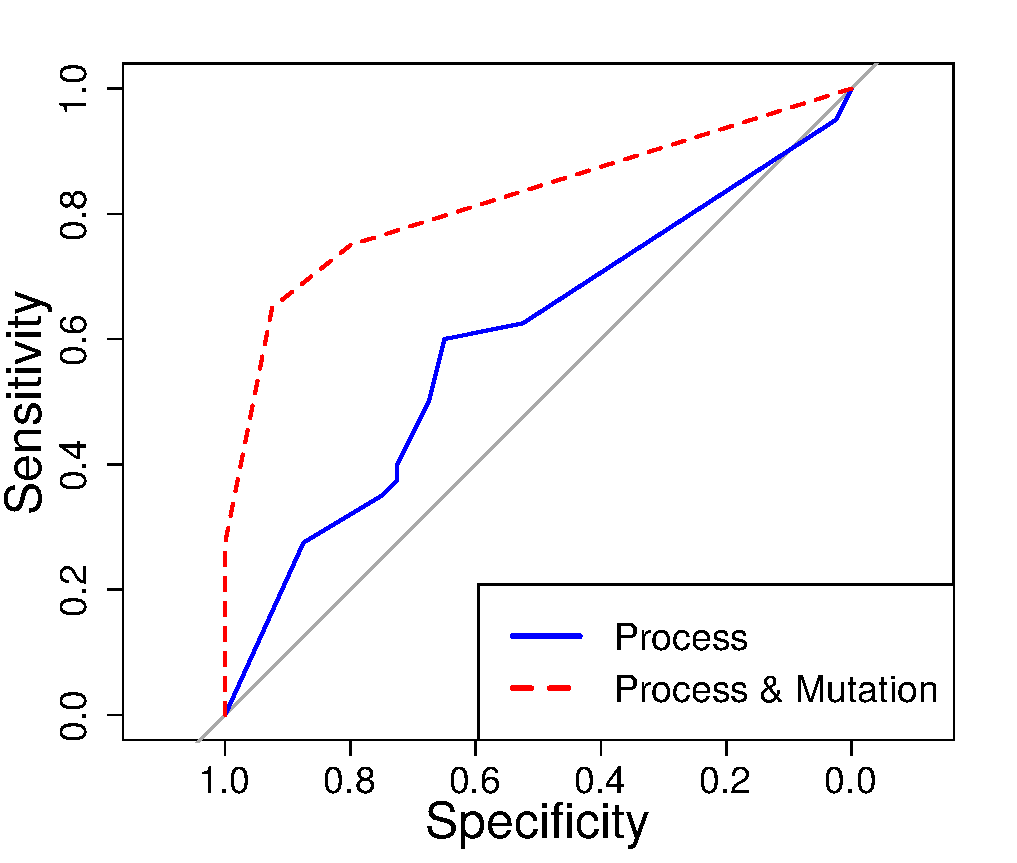
\includegraphics[width=\linewidth]{img/evaluation/phase1-roc-dt.pdf}
		\caption{\lr{Decition Tree}}
	\end{subfigure}
	\begin{subfigure}{.5\textwidth}
	\centering
	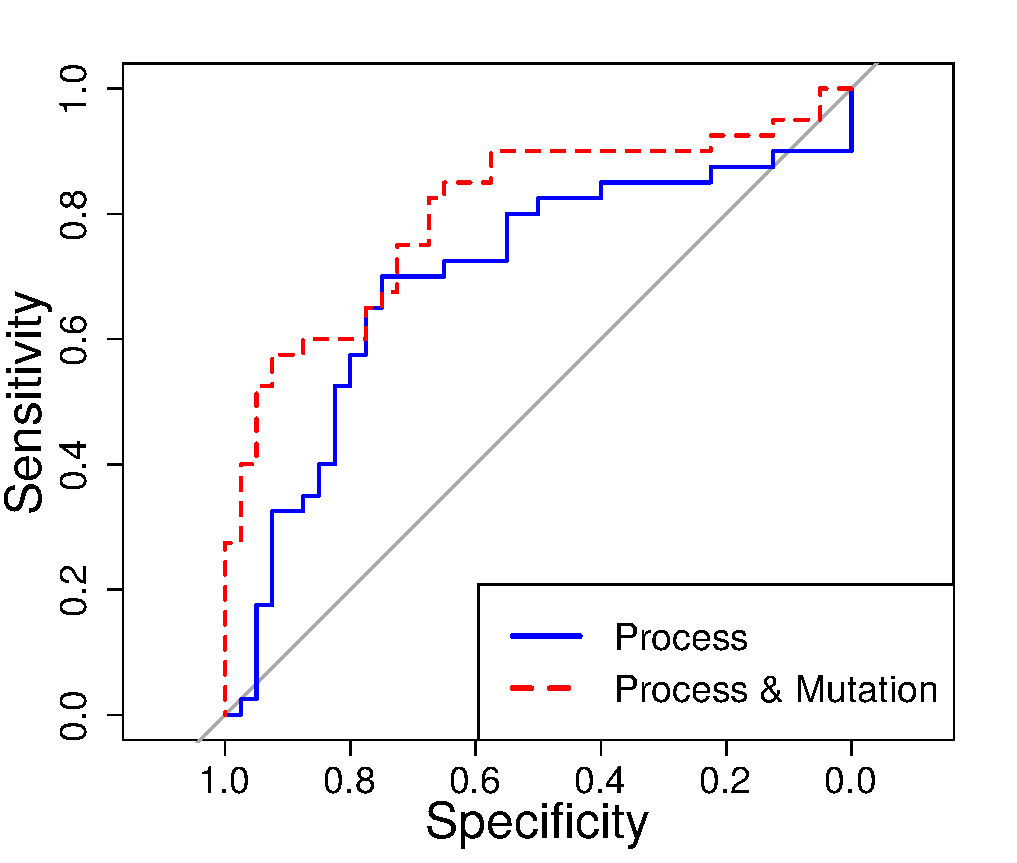
\includegraphics[width=\linewidth]{img/evaluation/phase1-roc-svm.pdf}
	\caption{SVM}
\end{subfigure}
	\begin{subfigure}{.5\textwidth}
	\centering
	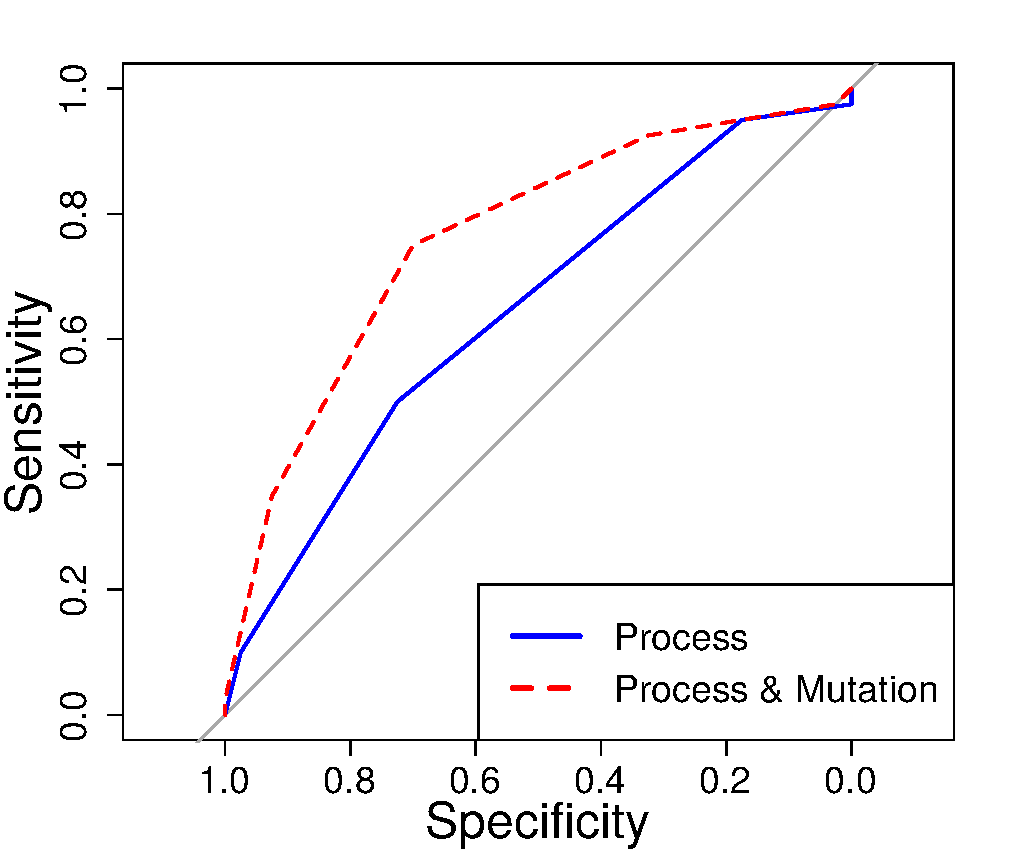
\includegraphics[width= \linewidth]{img/evaluation/phase1-roc-lr.pdf}
	\caption{\lr{Logestic Regression}}
\end{subfigure}
	\begin{subfigure}{.5\textwidth}
	\centering
	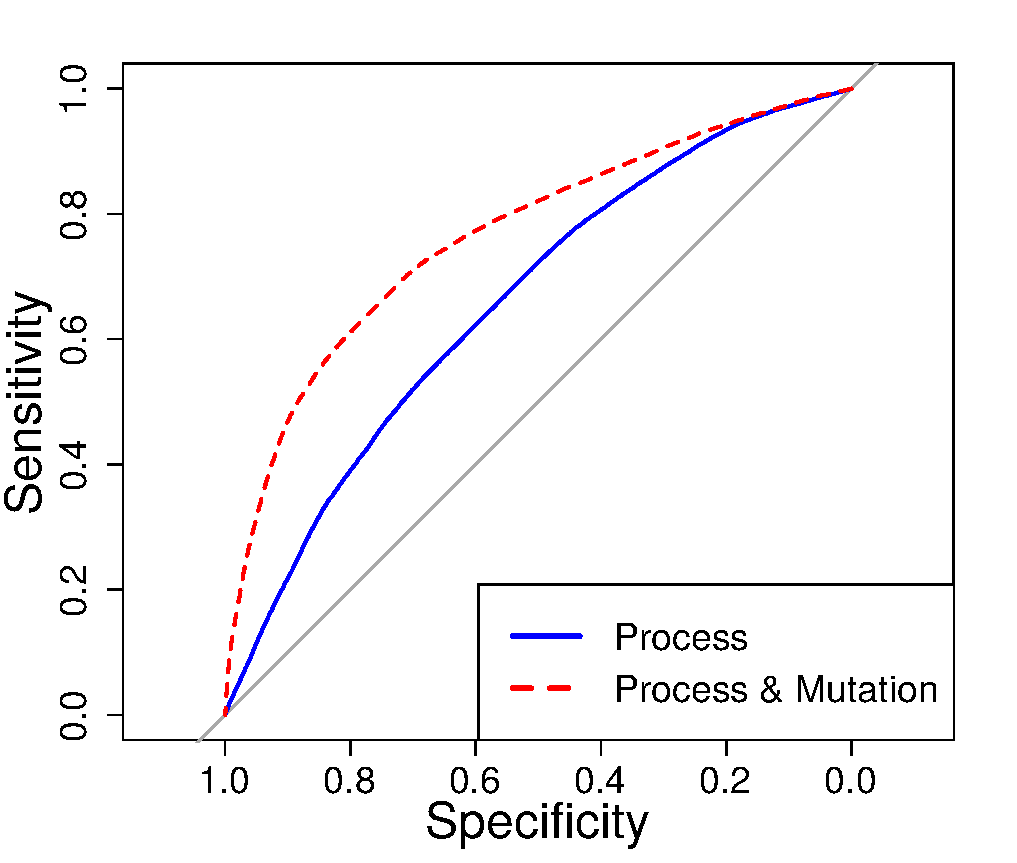
\includegraphics[width= \linewidth]{img/evaluation/phase1-roc-nn.pdf}
	\caption{\lr{Nueral Network}}
\end{subfigure}
\caption{نمودارهای ROC معیارهای فرآیند و به همراه جهش}
\label{fig:ROC-phase1}
\end{figure}

در جدول \ref{tab:auc-phase1} مساحت زیر نمودار ROC در هر یک از روش‌های دسته‌بندی آورده شده است.در میان  روش‌های یادگیری به کار گرفته شده بیشترین افزایش مساحت زیر نمودار را \lr{Neural Network} به مقدار $0.226$  واحد داشته است و کمترین  تغییر را نیز  \lr{Logestic Regression} با مقدار $0.038$ واحد داشته است.  به طور متوسط  $0.151$ واحد در مدلها بهبود مشاهده می‌شود. این موضوع نشان از تاثیر قابل توجه معیارهای جهش می‌باشد. 

\begin{table}[H] 
	\renewcommand*{\arraystretch}{1.2}	
	\centering \caption{مقادیر زیر نمودار ROC معیارهای فرآیند و به همراه جهش}
	\label{tab:auc-phase1}
	 \rowcolors{2}{blue!15}{white}   
	\begin{tabular}{|c|c|c|c|c|}
		\hline
		\hline
		معیار & 
		 \lr{ Decition Tree} & SVM &\lr{ Logestic Regression} &\lr{ Neural Network} \\
		 \hline
		 \hline
		 فرآیند & $.596$ & $.697$ & $.643$ & $.593$
		 \\
		 \hline
		 فرآیند و جهش  & $.822$ & $.802$ & $.761$ & $.829$
		 \\
		 \hline
		 
	\end{tabular}
\end{table}

\section{ارزیابی معیارهای فرآیند مبتنی بر جهش }
ارزیابی این معیارها در دو مرحله انجام می‌شود. در مرحله‌ی اول  سه  مدل ساخته می‌شود. این مدل‌ها به ترتیب با استفاده از معیارهای فرآیند، فرآیند و جهش و  مدل آخر با استفاده از معیارهای فرآیند و فرآیند مبتنی بر جهش ساخته می‌شود. در مرحله‌ی دوم دو  مدل ساخته می‌شود. در مدل اول معیارهای فرآیند و جهش مدل پیش‌بینی را خواهد ساخت و در مدل دوم معیارهای فرآیند مبتنی بر جهش نیز به مجموعه‌ی معیارها افزوده می‌شود. 

\subsection{مرحله‌ی اول}
 مقایسه‌ی این مدل‌ها امکان را فراهم می‌کند مشخص شود آیا معیارهای فرآیند مبتنی  بر جهش دارای قابلیت پیش‌بینی هستند یا خیر. همچنین در صورت داشتن این قابلیت مشخص شود که این قابلیت از معیارهای جهش کمتر است یا بیشتر. \\
 
مقایسه‌ی نتایج بدست آمده در جدول \ref{tab:eval-phase2-part1}  با جدول \ref{tab:eval-phase1} نشان می‌دهد که در تمامی روشهای دسته‌بندی  بجز SVM معیار صحت در مدل سوم از مدل اول مقدار بیشتری دارد.  در مدل ساخته شده توسط SVM نیز اختلاف معیار صحت کم می‌باشد(۳ درصد).  این مدل در مقایسه با مدل دوم عملکرد بهتری از نظر معیار صحت و بازخوانی در هیچکدام از روشهای دسته‌بندی نداشته است. از نظر معیار دقت  در  تمامی روشها مدل سوم از مدل اول عملکرد بهتری داشته و حتی در روش \lr{Decition Tree} مدل سوم از  مدل دوم نیز بهتر عملکرده است. از نظر معیار بازخوانی مدل سوم نسبت به مدل اول تنها در روش \lr{Neural Network} عملکرد بهتری داشته، در \lr{Decision Tree} بدون تغییر مانده و در دو روش دیگر کاهش یافته است. \\
می‌توان این نتیجه را برداشت کرد که معیارهای ارائه شده دارای توانایی پیش‌بینی بیشتری نسبت به معیارهای فرآیند به تنهایی هستند.
 \\
 \begin{table}[H] 
 	\renewcommand*{\arraystretch}{1.3}	
 	\centering \caption{نتایج پیش‌بینی‌خطای معیارهای فرآیند مبتنی بر جهش - مرحله‌ی اول} 
 	\label{tab:eval-phase2-part1}

 	\begin{tabular}{|c|c|c|c|}
 		
 		\hline
 		\hline
 		 نام روش  & صحت & دقت & بازخوانی	
 		\\
 		\hline
 		\hline
 		 
 		\lr{Decition Tree} & $0.725 $&$0.750$&$0.675$
 		\\
 		\hline
 	
 		\lr{SVM} & $0.637$&$0.689$&$0.500$
 		
 		\\
 		\hline
 	 
 		\lr{Logestic Regression} & $0.662$&$0.685$&$0.600$
 		\\
 		\hline
 	 
 		\lr{Neural Network} & $0.762$&$0.756$&$0.775$
 		\\
 		\hline
	\end{tabular}
 \end{table}

در شکل \ref{fig:ROC-phase2-part1} نمودارهای ROC سه مدل ساخته شده نشان داده شده است. در زیرشکل‌های (آ)(ج)(د) به وضوح عملکرد بهتر مدل سوم از مدل اول قابل مشاهده است. در زیرشکل (ب)نیز که متعلق به SVM است با رجوع به جدول \ref{tab:auc-phase2-part1} مشخص می‌شود که در این شکل نیز مساحت زیر نمودار ROC در مدل سوم بیشتر از اول است. همچنین مساحت زیر نمودار در مدل سوم در زیرشکل (ج) به مقدار $0.015$ واحد از مدل دوم نیز بیشتر است. 

این نتایج در راستای نتایج بدست آمده از جدول \ref{tab:eval-phase2-part1} می‌باشد. در نهایت می‌توان این نتیجه را گرفت که معیارهای مبتنی بر جهش معرفی شده دارای توانایی پیش‌بینی خطای بیشتری نسبت به معیارهای فرآیند هستند اما این توانایی بیشتر از معیارهای جهش نیست. همچنین از آنجا که هزینه‌ی محاسباتی بیشتری نسبت به معیارهای جهش دارند جایگزینی آنها به جای یکدیگر مزیتی ندارد. 

\begin{figure}[H]
	\begin{subfigure}{.5\textwidth}
		\centering
		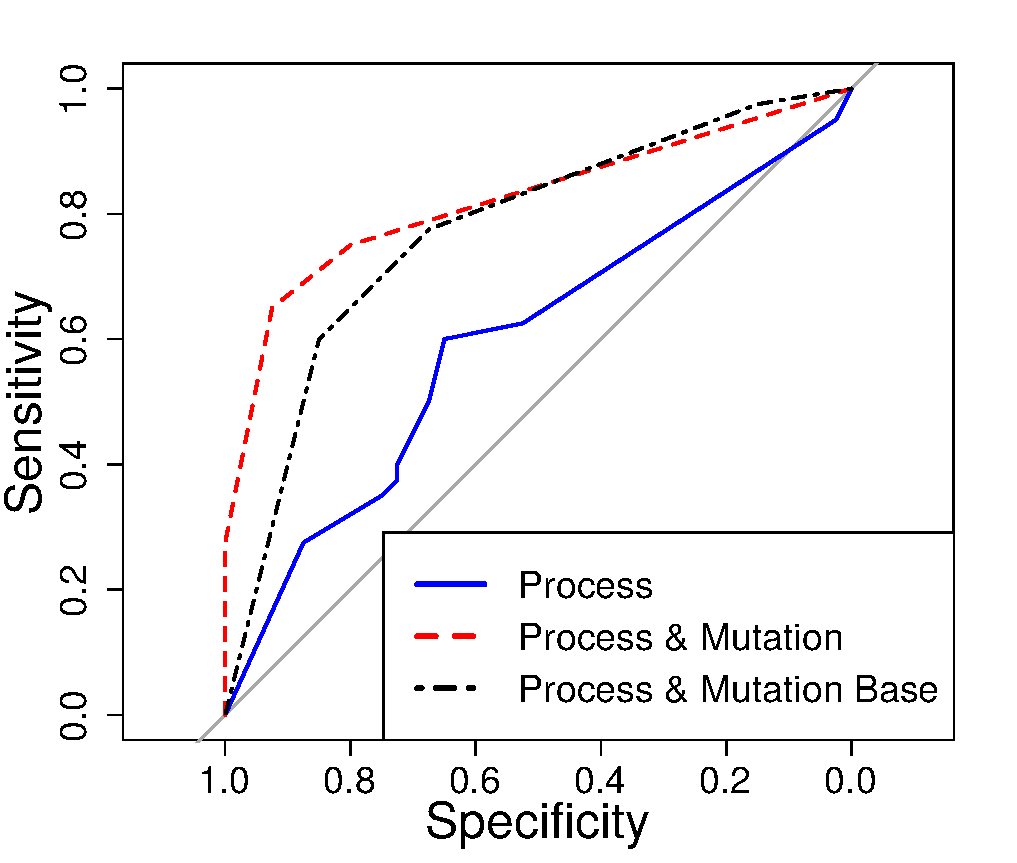
\includegraphics[width=\linewidth]{img/evaluation/phase2-part1-roc-dt.pdf}
		\caption{\lr{Decition Tree}}
	\end{subfigure}
	\begin{subfigure}{.5\textwidth}
		\centering
		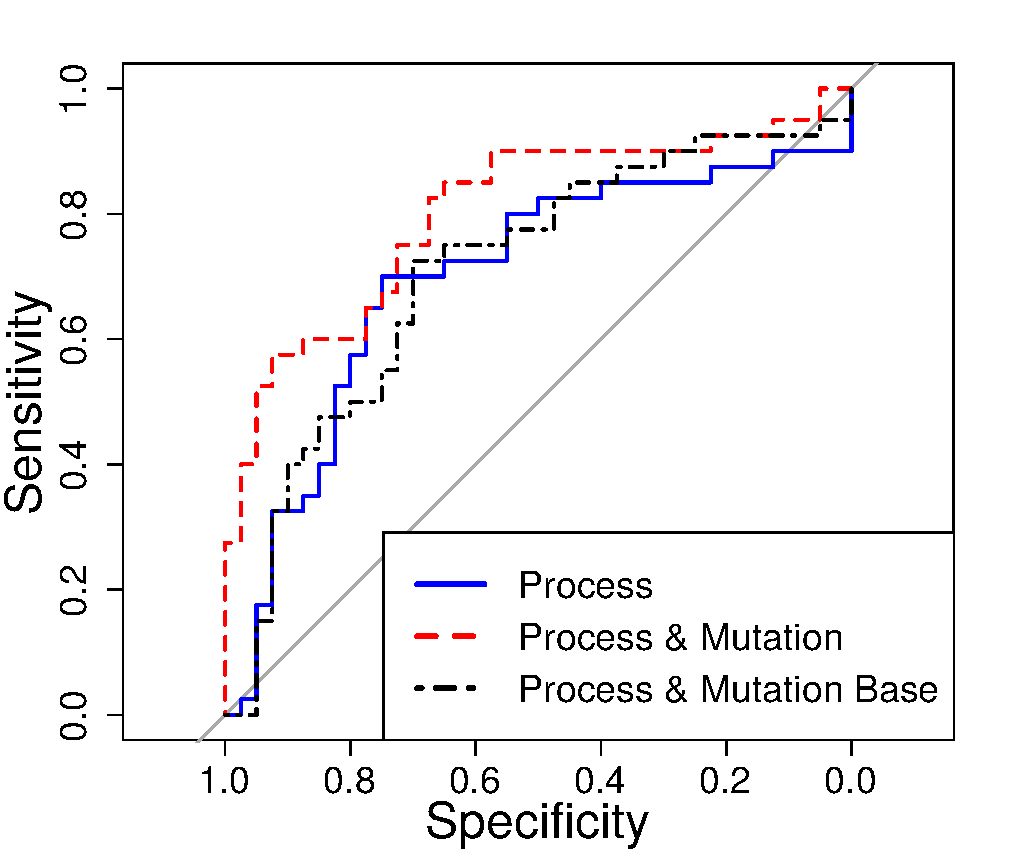
\includegraphics[width=\linewidth]{img/evaluation/phase2-part1-roc-svm.pdf}
		\caption{SVM}
	\end{subfigure}
	\begin{subfigure}{.5\textwidth}
		\centering
		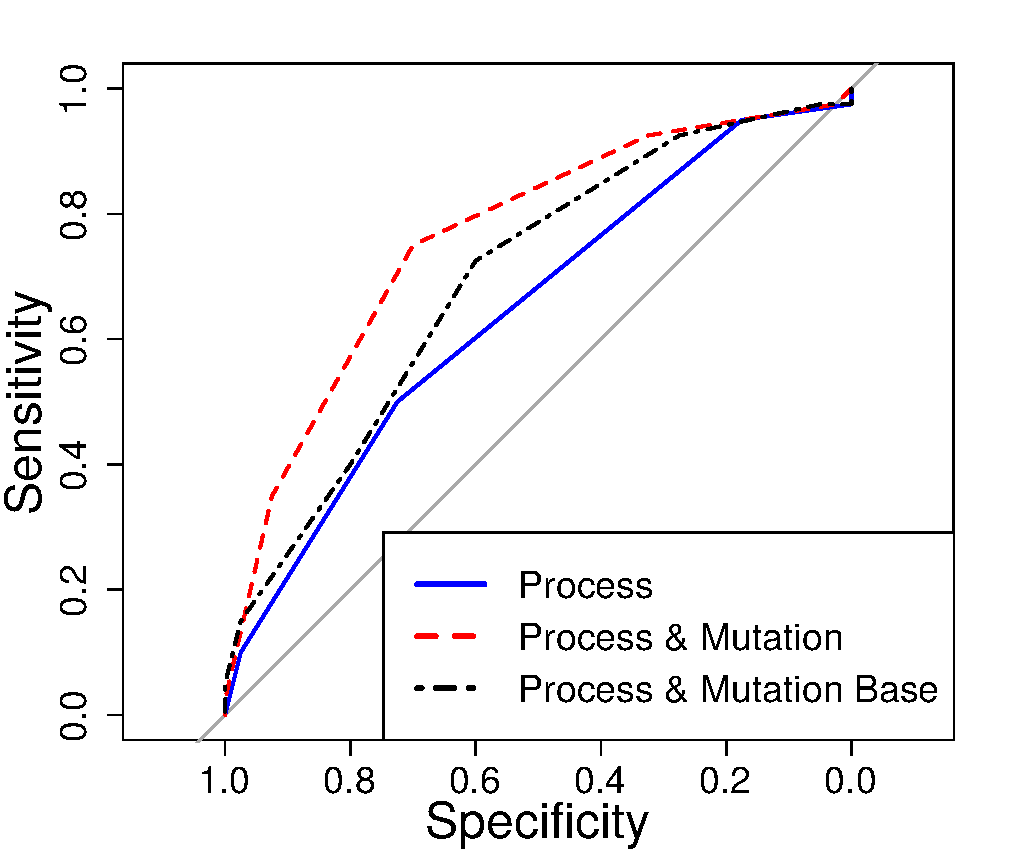
\includegraphics[width= \linewidth]{img/evaluation/phase2-part1-roc-lr.pdf}
		\caption{\lr{Logestic Regression}}
	\end{subfigure}
	\begin{subfigure}{.5\textwidth}
		\centering
		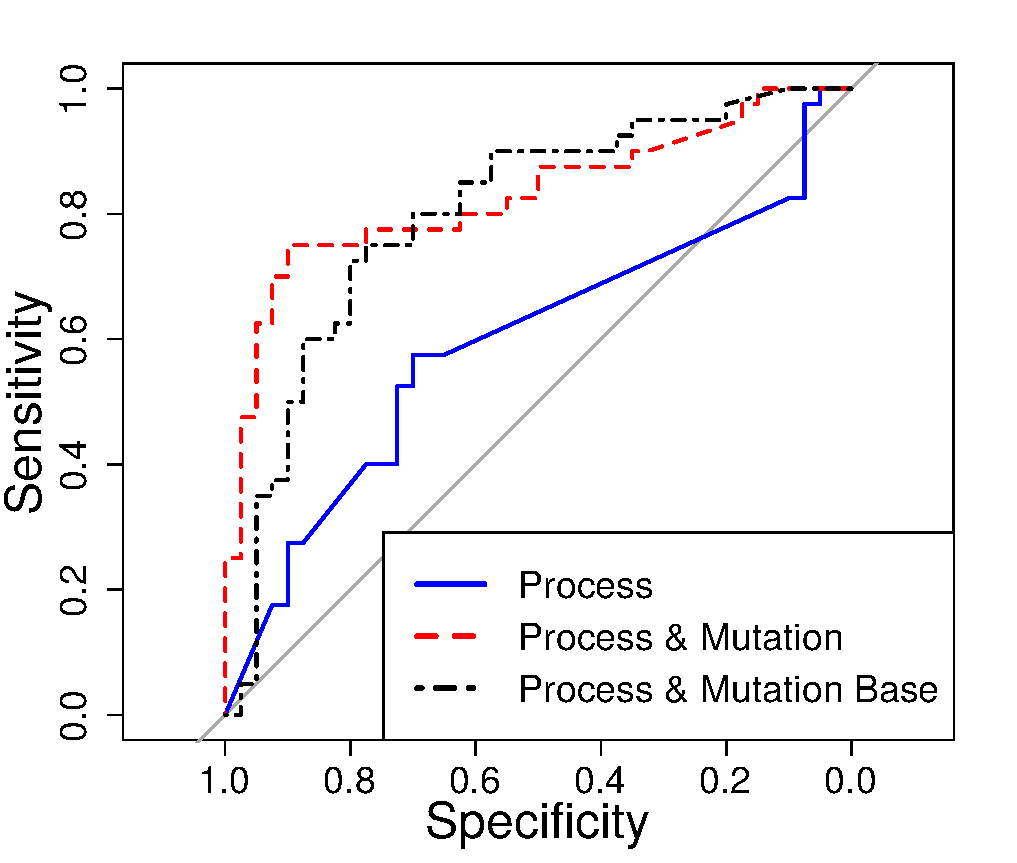
\includegraphics[width= \linewidth]{img/evaluation/phase2-part1-roc-nn.pdf}
		\caption{\lr{Nueral Network}}
	\end{subfigure}
	\caption{نمودارهای ROC معیارهای فرآیند ، فرآیند و جهش ، فرآیند مبتنی بر جهش}
	\label{fig:ROC-phase2-part1}
\end{figure}

\begin{table}[H] 
	\renewcommand*{\arraystretch}{1.2}	
	\centering \caption{مقادیر زیر نمودار ROC معیارهای فرآیند مبتنی جهش}
	\label{tab:auc-phase2-part1}
	\begin{tabular}{|c|c|c|c|}
		\hline
		\hline
		 
		\lr{ Decition Tree} & SVM &\lr{ Logestic Regression} &\lr{ Neural Network} \\
		\hline
		\hline
		 $.772$ & $.707$ & $.693$ & $.798$
		\\
		\hline
	
		
	\end{tabular}
\end{table}

\subsection{مرحله‌ی دوم}
همانطور که اشاره شد دو مدل ساخته می‌شود که مدل اول از معیارهای فرآیند و جهش استفاده می‌کند و مدل دوم همگی معیارها (با افزودن معیارهای فرآیند مبتنی بر جهش) در ساخت مدل استفاده می‌شود. هدف از این آزمایش این است که مشخص شود در صورتی که معیارهای ارائه شده‌ی جدید در کنار معیارهای قبلی قرار گیرد، در پیش‌بینی بهبودی حاصل می‌گردد یا خیر. 

نتایج بدست آمد در جدول \ref{tab:eval-phase2-part2} نشان می‌دهد که مدل دوم  در هیچ یک از روش‌ها بجز \lr{Logestic Regression} از نظر معیارهای صحت، دقت و بازخوانی نسبت به مدل اول بهبودی پیدا نکرده است. همچنین در روش \lr{Decition Tree} نتایج دو مدل یکسان است.  در روش \lr{Logestic Regression} مدل دوم در معیار صحت $1.2$ درصد افزایش، در معیار دقت $5$ درصد کاهش و $17.5$ درصد، بازخوانی افزایش داشته است. 

 \begin{table}[H] 
	\renewcommand*{\arraystretch}{1.3}	
	\centering \caption{نتایج پیش‌بینی خطای مدل حاصل از بکارگیری تمامی معیارها}
	\label{tab:eval-phase2-part2}
	
	\begin{tabular}{|c|c|c|c|}
		
		\hline
		\hline
		نام روش  & صحت & دقت & بازخوانی	
		\\
		\hline
		\hline
		
		\lr{Decition Tree} & $0.787$&$0.725$&$0.925$
		\\
		\hline
		
		\lr{SVM} & $0.712$&$0.774$&$0.600$
		\\
		\hline
		
		\lr{Logestic Regression} & $0.737 $&$0.686$&$0.875$
		\\
		\hline
		
		\lr{Nueral Network} & $0.750$&$0.717$&$0.825$
		\\
		\hline
	\end{tabular}
\end{table}
 
 نمودارهای ROC هر یک از این دو مدل در روش‌های دسته‌بندی مختلف در شکل \ref{fig:ROC-phase2-part2} آمده است. در روش‌های مختلف مدل اول با دوم تفاوت چندانی ندارند و طبق جدول \ref{tab:auc-phase2-part2} تنها در مدل‌های حاصل از روش \lr{Logestic Regression} به مقدار $0.009$ واحد مساحت زیر نمودار افزایش پیدا  کرده است. بنابرین قرار گیری معیارهای فرآیند مبتنی بر جهش نمی‌تواند به بهبود پیش‌بینی بیانجامد.
\begin{figure}[H]
	\begin{subfigure}{.5\textwidth}
		\centering
		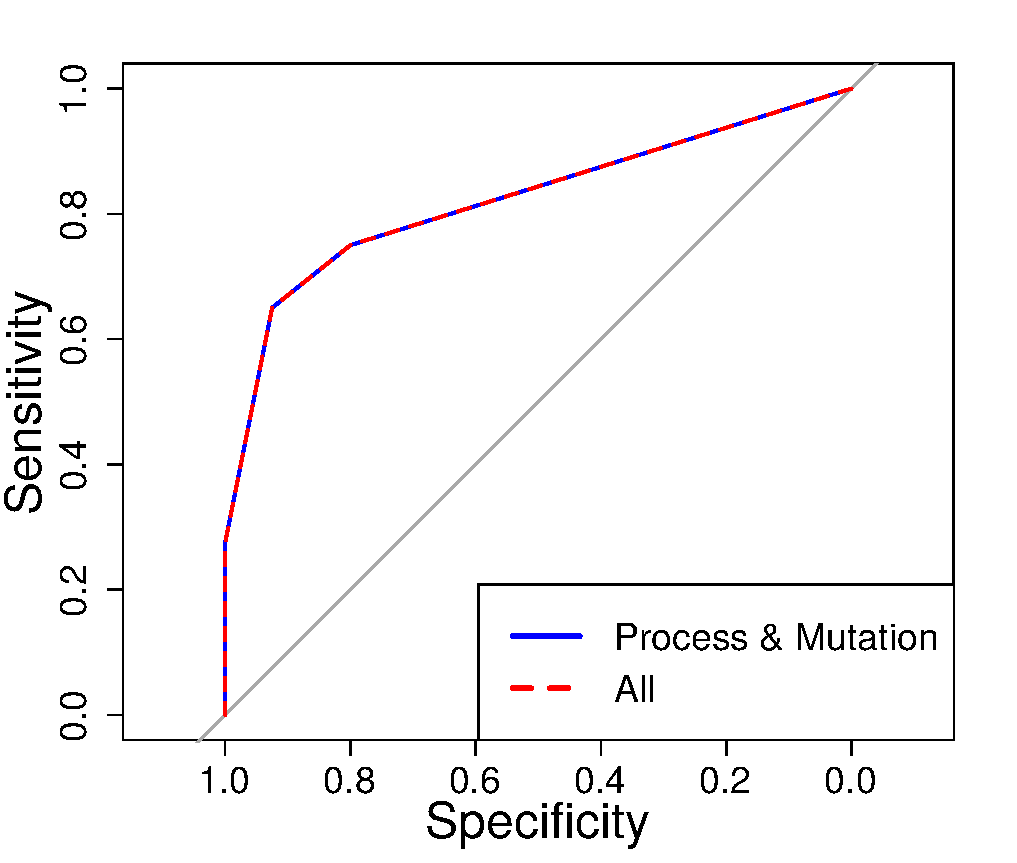
\includegraphics[width=\linewidth]{img/evaluation/phase2-part2-roc-dt.pdf}
		\caption{\lr{Decition Tree}}
	\end{subfigure}
	\begin{subfigure}{.5\textwidth}
		\centering
		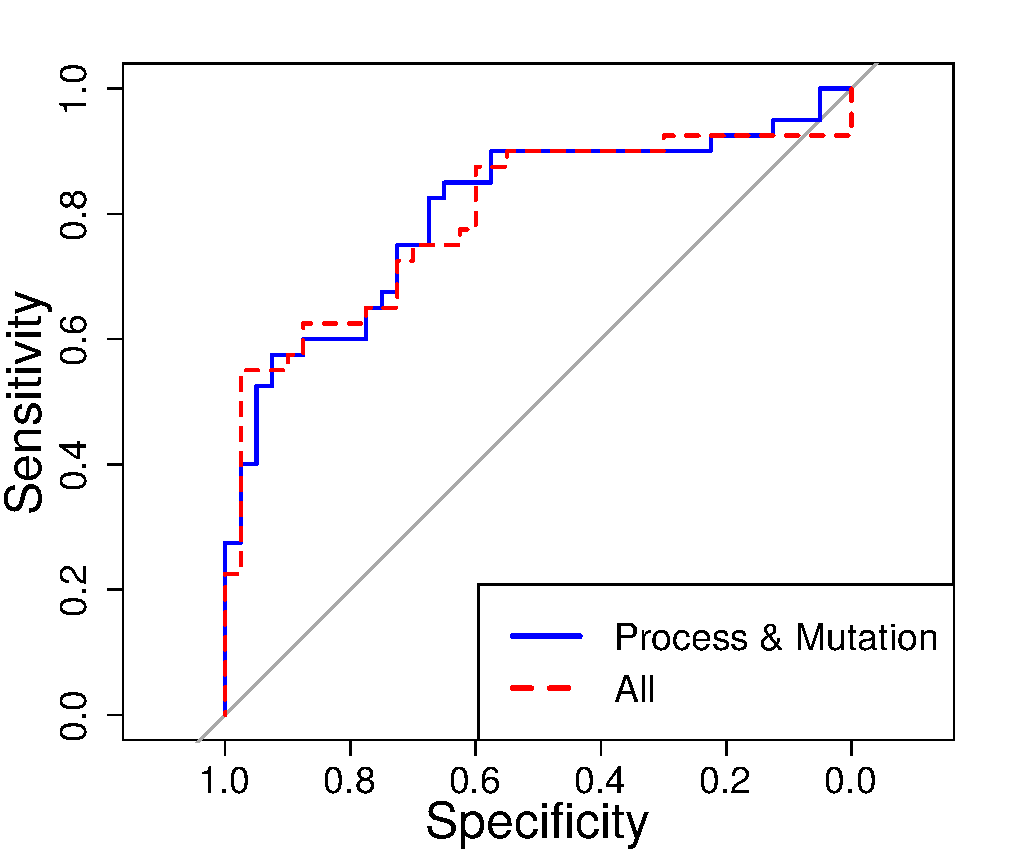
\includegraphics[width=\linewidth]{img/evaluation/phase2-part2-roc-svm.pdf}
		\caption{SVM}
	\end{subfigure}
	\begin{subfigure}{.5\textwidth}
		\centering
		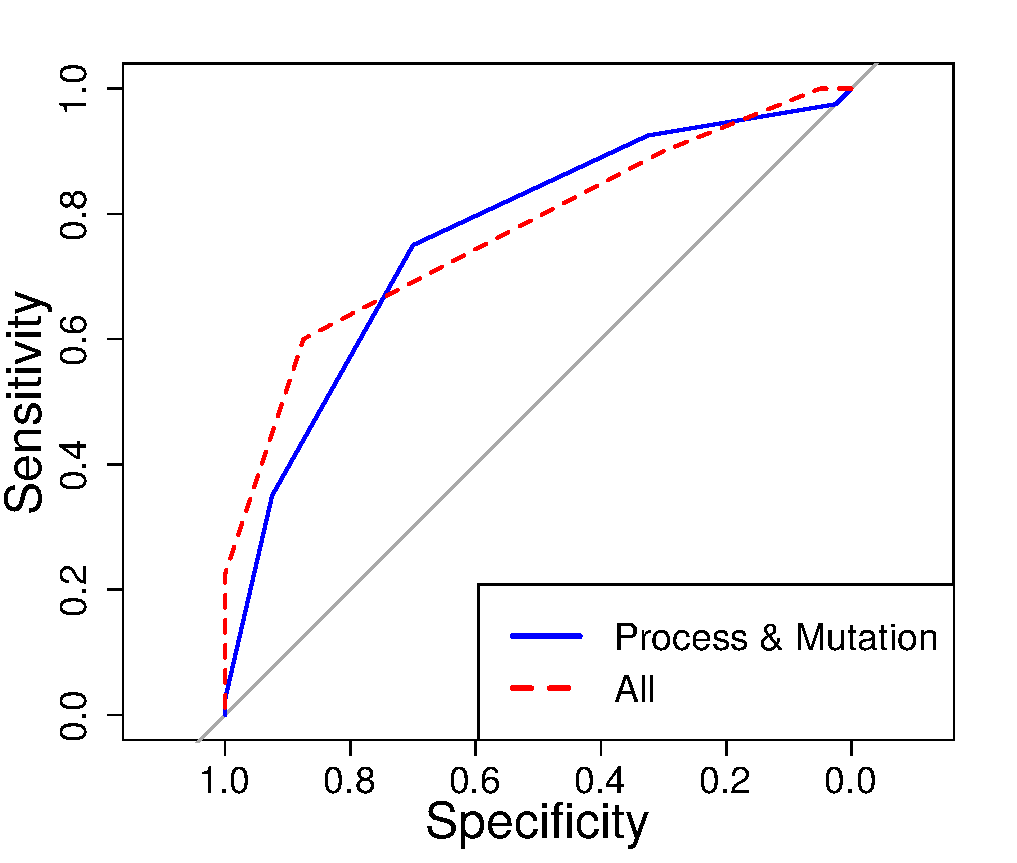
\includegraphics[width= \linewidth]{img/evaluation/phase2-part2-roc-lr.pdf}
		\caption{\lr{Logestic Regression}}
	\end{subfigure}
	\begin{subfigure}{.5\textwidth}
		\centering
		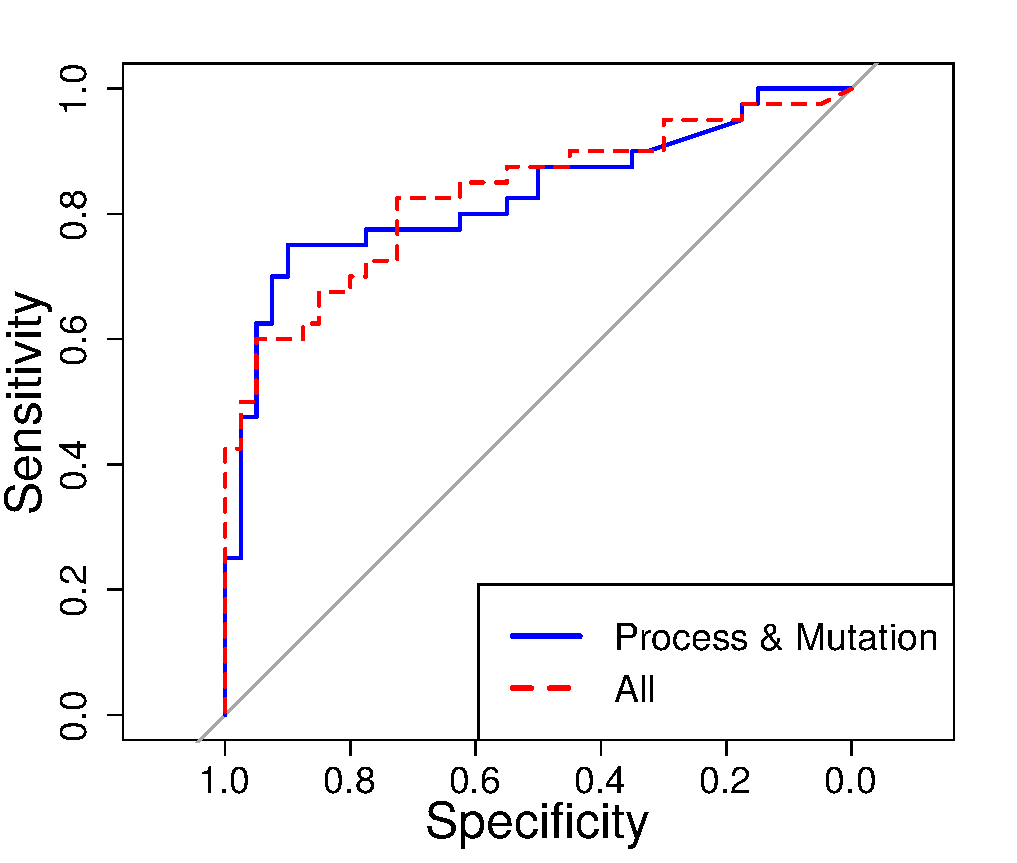
\includegraphics[width= \linewidth]{img/evaluation/phase2-part2-roc-nn.pdf}
		\caption{\lr{Nueral Network}}
	\end{subfigure}
	\caption{نمودارهای ROC معیارهای جهش و فرآیند و تمامی معیارها }
	\label{fig:ROC-phase2-part2}
\end{figure}

\begin{table}[H] 
	\renewcommand*{\arraystretch}{1.2}	
	\centering \caption{مقادیر زیر نمودار ROC تمامی معیارها}
	\label{tab:auc-phase2-part2}
	\begin{tabular}{|c|c|c|c|}
		\hline
		\hline
		
		\lr{ Decition Tree} & SVM &\lr{ Logestic Regression} &\lr{ Neural Network} \\
		\hline
		\hline
		$.822$ & $.786$ & $.770$ & $.830$
		\\
		\hline
		
		
	\end{tabular}
\end{table}

\section{ارزیابی معیارهای ترکیبی فرآیند-جهش}
 در این قسمت به ارزیابی دو معیار مطرح شده پرداخته می‌شود. به منظور ارزیابی آنها دو مدل با استفاده از هر یک از روشهای انتخابی استفاده می‌شود. در مدل اول معیارهای فرآیند استفاده می‌شود و در مدل دوم معیار \موکد{مقدار نرمال شده‌ی خطوط اضافه شده} با معیار \موکد{تعداد خطوط اضافی وزن‌دهی شده} جایگزین می‌شود و معیار \موکد{مقدار نرمال شده‌ی خطوط حذف شده} به طور مشابه جایگزین می‌شود. سایر معیارهای مدل دوم با مدل اول یکسان خواهد بود.

 نتایج به دست آمده در جدول \ref{tab:eval-phase3} نشان می‌دهد که معیارهای صحت، دقت و بازخوانی برای تمامی مدل‌ها بجز مدل ساخته شده توسط روش SVM افزایش قابل ملاحظه‌ای داشته است. بیشترین افزایش صحت در روش \lr{Neural Network} به میزان $13.8$ درصد روی داده است. از نظر افزایش دقت بیشترین تغییر مثبت در روش \lr{Decition Tree} بوده است که $13.1$ درصد رشد داشته است. معیار بازخوانی در دو  روش \lr{Logestic Regression} و \lr{Neural Network} به ترتیب $8.4$ و $2.5$ رشد داشته و در دو روش دیگر کاهش داشته است. \\
 به طور میانگین معیار صحت $6.6$ درصد افزایش، معیار دقت $6$ درصد افزایش  و معیار بازخوانی $0.4$ درصد کاهش داشته است. در نهایت می‌توان این نتیجه را گرفت که معیارهای ترکیبی جهش-فرآیند موجب بهبود در صحت و دقت پیش‌بینی می‌شوند و تاثیر چندانی در بازخوانی ندارند. لازم به ذکر است که تنها دو معیار از ۱۲ معیار مورد استفاده در دو مدل ساخته شده با هم متفاوت هستند که این دو معیار توانسته‌اند حدود $6$ درصد صحت و دقت را بهبود بخشند. این امر نشان از تاثیر قابل ملاحظه‌ی این معیارها می‌باشد. \\
 



\begin{table}[H] 
	\renewcommand*{\arraystretch}{1.3}	
	\centering \caption{مقایسه‌ی معیارهای فرآیند و معیارهای ترکیبی جهش-فرآیند}
	\label{tab:eval-phase3}
	\rowcolors{2}{blue!15}{white}   
	\begin{tabular}{|c|c|c|c|c|}
		
		\hline
		\hline
		معیار & نام روش  & صحت & دقت & بازخوانی	
		\\
		\hline
		\hline
		فرآیند & 
		\lr{Decition Tree} & $0.587$&$0.574$&$0.675$
		\\
		\hline
		ترکیبی جهش-فرآیند& 
		\lr{Decition Tree} & $0.675$&$0.705$&$0.600$
		\\
		\hline
		فرآیند & 
		\lr{SVM} & $0.662$&$0.685$&$0.600$
		\\
		\hline
		ترکیبی جهش-فرآیند & 
		\lr{SVM} & $0.637$&$0.666$&$0.550$
		\\
		
		\hline
		فرآیند &
		\lr{Logestic Regression} & $0.612$&$0.591$&$0.725$
		\\
		\hline
		ترکیبی جهش-فرآیند & 
		\lr{Logestic Regression} & $0.675 $&$0.652$&$0.750$
		\\
		\hline
		فرآیند &
		\lr{Nueral Network} & $0.612$&$0.725$&$0.591$
		\\
		\hline
		ترکیبی جهش-فرآیند & 
		\lr{Nueral Network} & $0.750$&$0.794$&$0.675$
		\\
		\hline		
	\end{tabular}
\end{table}

در شکل \ref{fig:ROC-phase3} نمودارهای ROC به تفکیک روش دسته‌بندی آمده است. در هر یک از زیر شکل‌ها منحنی ROC مربوط به  دو مدل با هم مقایسه شده است. درمدل اول که در ساخت آن از معیارهای فرآیند استفاده شده  با خط ممتد نمایش داده شده است و مدل دوم  از جایگزینی دو معیار فرآیند با معیارهای ترکیبی جهش-فرآیند ساخته شده و با خط چین نمایش داده شده‌. همانطور که قابل مشاهده است در تمامی روش‌ها بجز  SVM مدل‌ دوم مساحت زیر نمودار بیشتری نسبت به مدل اول داشته است.
\begin{figure}[H]
	\begin{subfigure}{.5\textwidth}
		\centering
		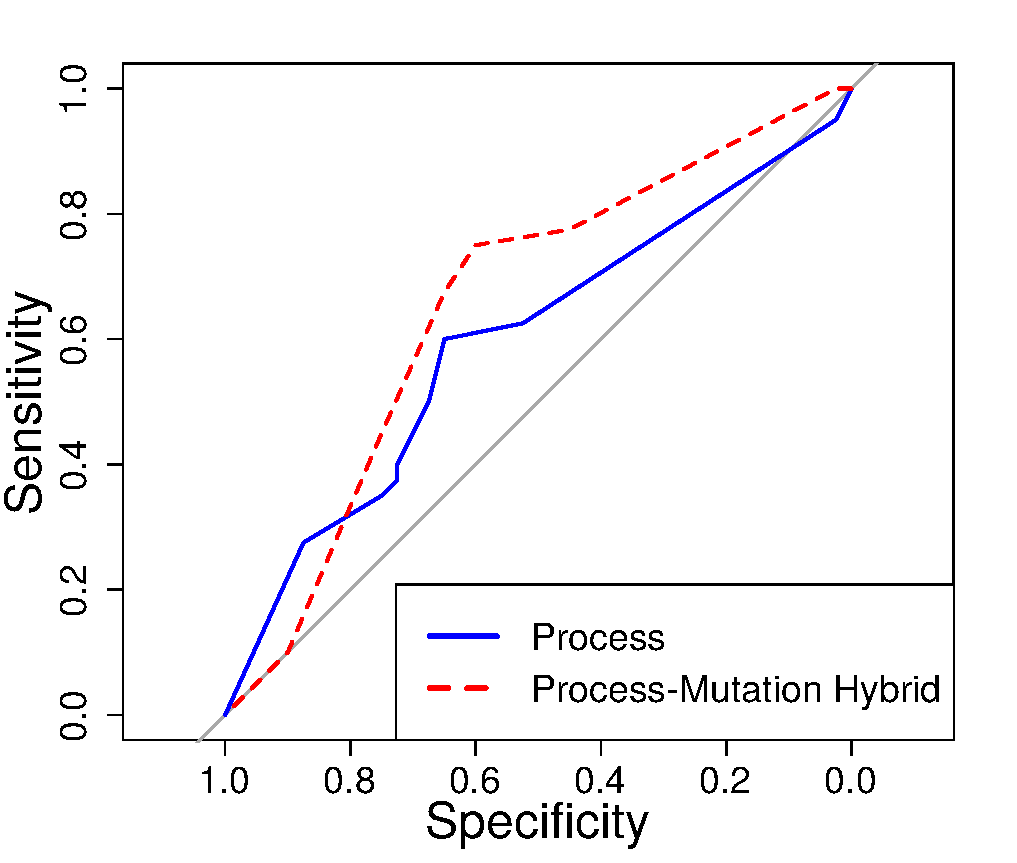
\includegraphics[width=\linewidth]{img/evaluation/phase3-roc-dt.pdf}
		\caption{\lr{Decition Tree}}
	\end{subfigure}
	\begin{subfigure}{.5\textwidth}
		\centering
		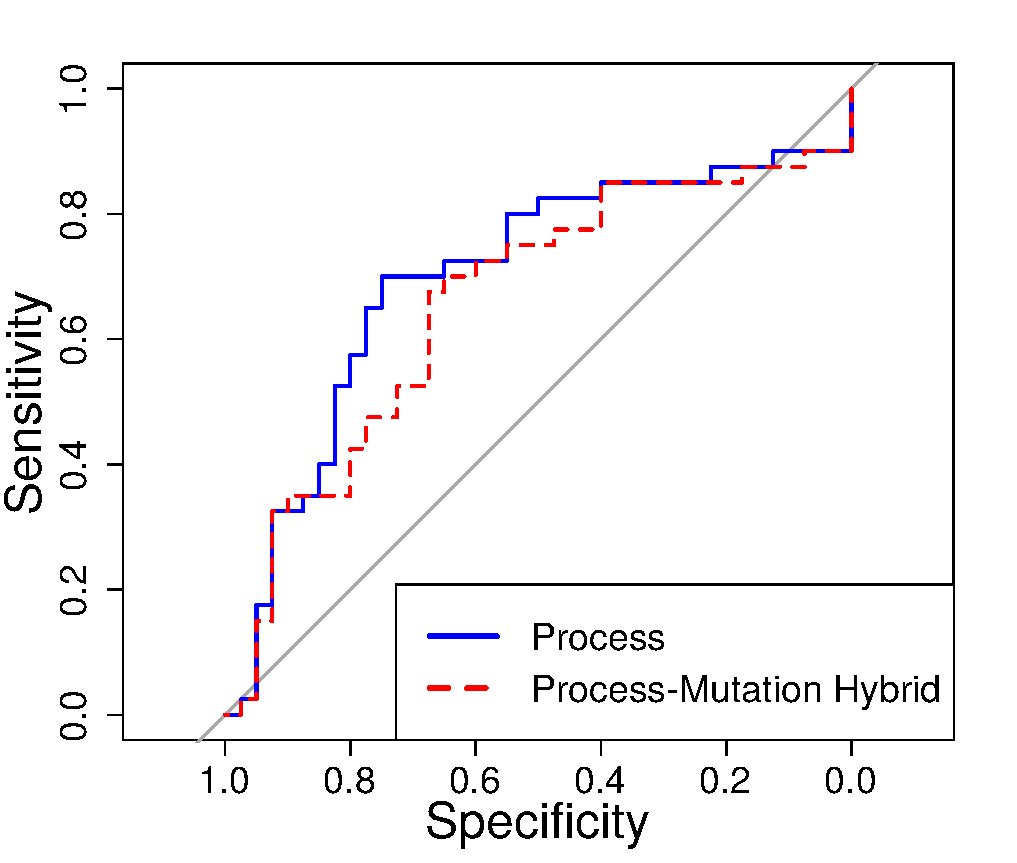
\includegraphics[width=\linewidth]{img/evaluation/phase3-roc-svm.pdf}
		\caption{SVM}
	\end{subfigure}
	\begin{subfigure}{.5\textwidth}
		\centering
		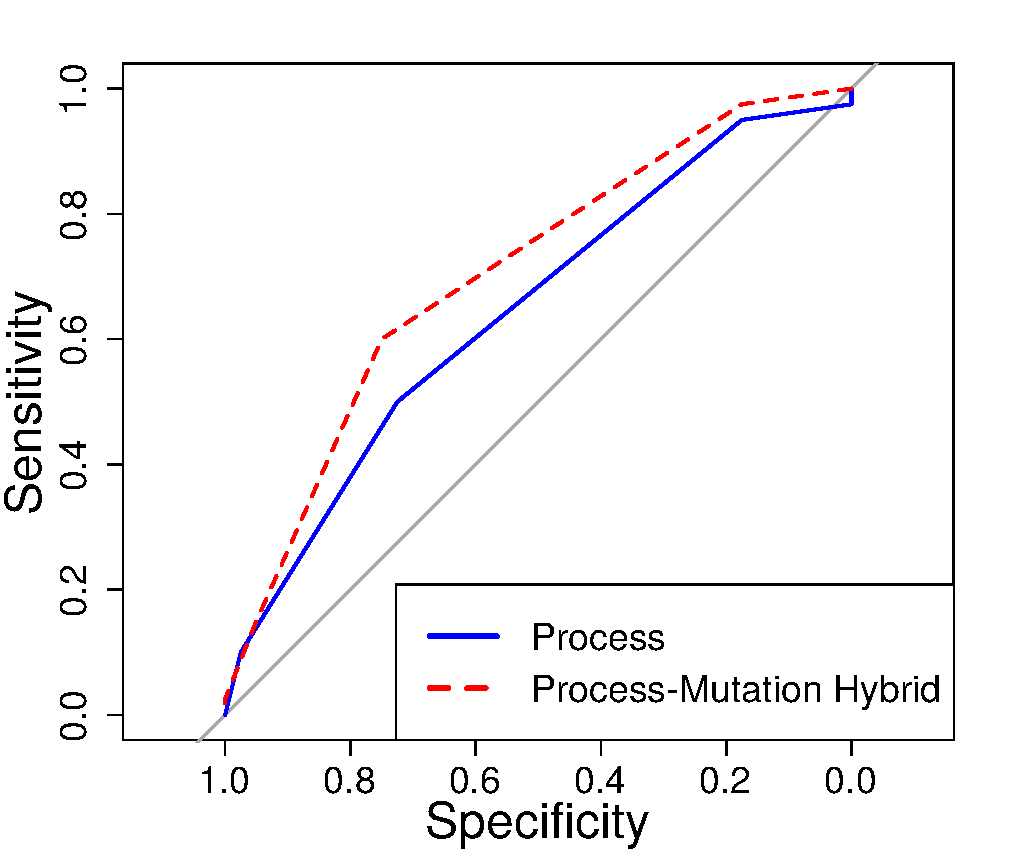
\includegraphics[width= \linewidth]{img/evaluation/phase3-roc-lr.pdf}
		\caption{\lr{Logestic Regression}}
	\end{subfigure}
	\begin{subfigure}{.5\textwidth}
		\centering
		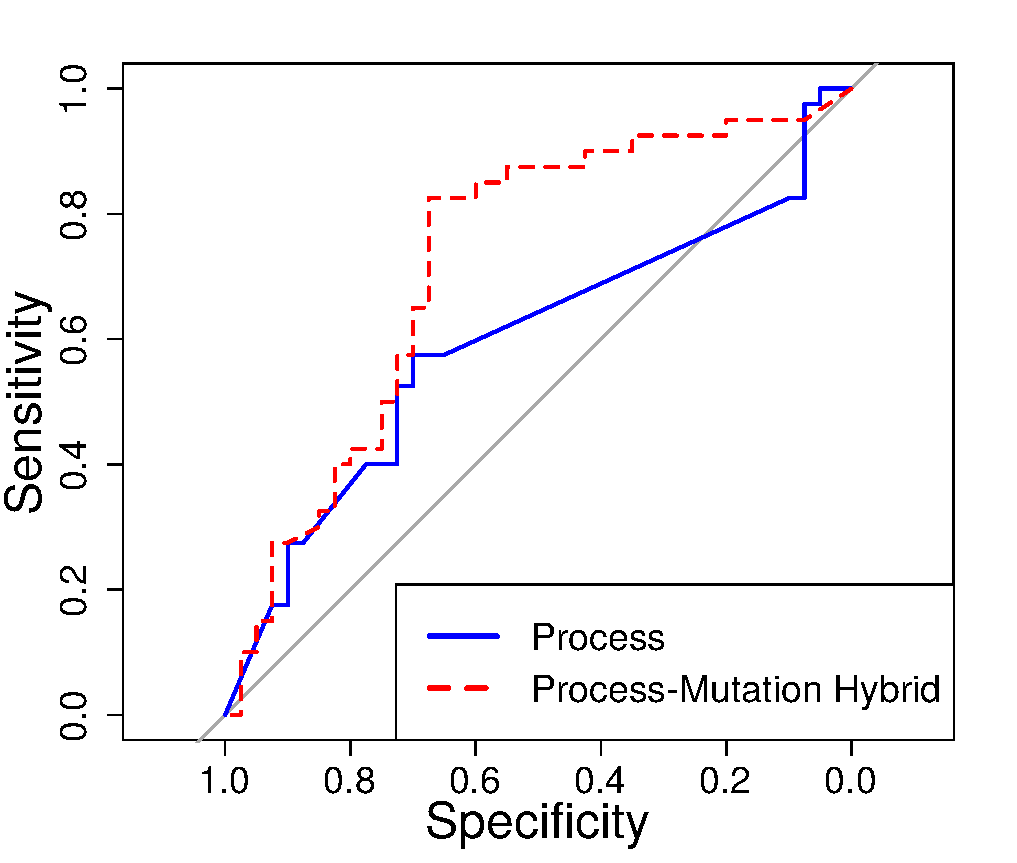
\includegraphics[width= \linewidth]{img/evaluation/phase3-roc-nn.pdf}
		\caption{\lr{Nueral Network}}
	\end{subfigure}
	\caption{نمودارهای ROC معیارهای فرآیند و به همراه جهش}
	\label{fig:ROC-phase3}
\end{figure}

در جدول \ref{tab:auc-phase3} مساحت زیر نمودار ROC  دو مدل به تفکیک روش دسته‌بندی آورده شده است. در میان  روش‌های یادگیری به کار گرفته شده بیشترین افزایش مساحت زیر نمودار را روش  \lr{Neural Network} به مقدار $0.128$  واحد داشته است. به طور متوسط  $0.051$ واحد در مدل‌ها بهبود مشاهده می‌شود. این موضوع نشان می‌دهد که معیارهای ترکیبی جهش-فرآیند از نظر مساحت زیر نمودار ROC نیز موجب تغییر مثبت ایجاد می‌کند. \\

با توجه به اینکه تنها روش SVM  نتایج ضعیفی نسبت به سایرین داشته است این موضوع را می‌توان با توجه نحوه‌ی عملکرد این روش توجیه کرد. به طور خلاصه این روش سعی می‌کند که  \واژه{فضای ویژگی}  را با ایجاد یک \واژه{ابرصفحه} به دسته‌های مختلف تقسیم کند اما توزیع نقاط داده در فضای ویژگی به نحوی نیست که این روش بتواند به خوبی عمل کند. 

\begin{table}[H] 
	\renewcommand*{\arraystretch}{1.2}	
	\centering \caption{مقادیر زیر نمودار ROC معیارهای فرآیند و معیارهای ترکیبی جهش-}
	\label{tab:auc-phase3}
	\rowcolors{2}{blue!15}{white}   
	\begin{tabular}{|c|c|c|c|c|}
		\hline
		\hline
		معیار & 
		\lr{ Decition Tree} & SVM &\lr{ Logestic Regression} &\lr{ Neural Network} \\
		\hline
		\hline
		فرآیند & $.596$ & $.697$ & $.643$ & $.593$
		\\
		\hline
		جهش-فرآیند  & $.654$ & $.656$ & $.705$ & $.721$
		\\
		\hline
		
	\end{tabular}
\end{table}